\documentclass{tufte-handout}

\title{Math 451, Homework Set \#2}
\author{Anthony Brice}

\usepackage{pgfplots} % nice graphs

\usepackage{graphicx} % allow embedded images
\setkeys{Gin}{width=\linewidth,totalheight=\textheight,keepaspectratio}
% \graphicspath{{graphics/}} % set of paths to search for images
\usepackage{amsmath, amsthm, amssymb, amsfonts}  % extended mathematics
\usepackage{booktabs} % book-quality tables
\usepackage{units}    % non-stacked fractions and better unit spacing
\usepackage{multicol} % multiple column layout facilities
\usepackage{lipsum}   % filler text
\usepackage{fancyvrb} % extended verbatim environments
  \fvset{fontsize=\normalsize}% default font size for fancy-verbatim
                              % environments
% Standardize command font styles and environments
\newcommand{\doccmd}[1]{\texttt{\textbackslash#1}}% command name -- adds backslash automatically
\newcommand{\docopt}[1]{\ensuremath{\langle}\textrm{\textit{#1}}\ensuremath{\rangle}}% optional command argument
\newcommand{\docarg}[1]{\textrm{\textit{#1}}}% (required) command argument
\newcommand{\docenv}[1]{\textsf{#1}}% environment name
\newcommand{\docpkg}[1]{\texttt{#1}}% package name
\newcommand{\doccls}[1]{\texttt{#1}}% document class name
\newcommand{\docclsopt}[1]{\texttt{#1}}% document class option name
\newenvironment{docspec}{\begin{quote}\noindent}{\end{quote}}% command
                                % specification environment
\newcommand{\e}[1]{\ensuremath{\times 10^{#1}}} % Macro for scientific notation
\usepackage{enumitem} % nice lists

\usepackage{mathtools}
\DeclarePairedDelimiter\abs{\lvert}{\rvert}%
\DeclarePairedDelimiter\norm{\lVert}{\rVert}%
\renewcommand\Re{\operatorname{Re}}
\renewcommand\Im{\operatorname{Im}}
\newcommand\Arg{\operatorname{Arg}}


% Use fancy symbols for footnotes
\usepackage{hyperref}
\usepackage{natbib}
\renewcommand{\thefootnote}{\fnsymbol{footnote}}
\usepackage{perpage}
\MakePerPage{footnote}

\begin{document}

\maketitle

\section{Exercise 1}

\textit{Apply de Moivre's theorem to
  ${(\cos \theta + i \sin \theta)}^3$ and equate real and imaginary
  parts to derive trigonometric identities for $\cos(3\theta)$ and
  $\sin(3\theta)$.}

\bigskip

We begin by restating de Moivre's theorem: Let
$w = r( \cos \alpha + i \sin \alpha) = re^{i \alpha}$. Then
$w^n = r^n (\cos( n \alpha) + i \sin( n \alpha)) = r^n e^{ i n
  \alpha}$.

By expanding the polynomial we get%
\[ {(\cos \theta + i \sin \theta)}^3 = \cos^3 \theta - 3 \cos \theta
\sin^2 \theta + i (3 \cos^2 \theta \sin \theta - \sin^3 \theta),\]
and by de Moivre's theorem%
\[{(\cos \theta + i \sin \theta)}^3 = \cos( 3 \theta ) + i \sin( 3
\theta ).\]

Then equating the real and imaginary parts of the previous two
equations yields%
\begin{align*}
  \cos ( 3 \theta) &= \cos^3 \theta - 3 \cos \theta \sin^2 \theta\\
  \sin( 3 \theta) &= 3 \cos^2 \theta \sin \theta - \sin^3 \theta.\\
\end{align*}

\section{Exercise 2}

\textit{Show that if $\omega \neq 1$ is an $n$-th root of unity, then
  $1 + \omega + \omega^2 + \dots + \omega^{n - 1} = 0$. Hint: An
  $n$-th root of unity satisfies $z^n - 1 = 0$. Now, factor out $z -
  1$.}

\bigskip

Consider that via synthetic division we have that%
\[ z^n + 1 = (z - 1)\left( z^{n - 1} + z^{n - 2} + \cdots + z + 1 \right) .\]

Then%
\[ a + ar + ar^2 + \cdots + ar^n = {a \left(1 - r^{n + 1}\right) \over 1 - r} \]
if $r \neq 1$.

Let $z = \omega$, $\omega \neq 1$, then%
\[ \omega^{n - 1} + \cdots + \omega + 1 = 0. \]

\section{Exercise 3}

\textit{Given $z_1, z_2 \in \mathbb{C}$, solve
  $z_1 w_1 - z_2 \overline{w_2} = 1$ and
  $z_1 w_2 + z_2 \overline{w_1} = 0$ for $w_1$ and $w_2$. Using
  properties of conjugates may be useful!}

Solving for $w_1$ and $w_2$,

\begin{equation*}
\begin{aligned}
  (\overline{z_1}\overline{w_1} - z_2 w_2 = 1) &\cdot z_1\\
  + \; (z_2 \overline{w_1} + z_1 w_2 = 0) &\cdot \overline{z_2}\\
  \midrule
  (z_1 \overline{z_1})w_1 + (z_2 \overline{z_2})\overline{w_1} + 0 &= z_1.
\end{aligned}
\end{equation*}

Therefore
\begin{align*}
  &(z_1 \overline{z_1} + z_2 \overline{z_2})w_1 = z_1\\
  \Rightarrow &\left( \abs{z_1}^2 + \abs{z_2}^2 \right)\overline{w_1}
                                               = z_1\\
  \Rightarrow &w_1 = {z_1 \over \abs{z_1}^2 + \abs{z_2}^2}.
\end{align*}

And from our second equation
\begin{align*}
  w_2 &= -{z_2 \overline{w_1} \over z_1}\\
      &= -{z_2 \over z_1} \cdot {z_1 \over \abs{z_1}^2 + \abs{z_2}^2}\\
      &= -{z_2 \over \abs{z_1}^2 + \abs{z_2}^2}.
\end{align*}

\section{Exercise 4}

\textit{First, show that any root of unity lies on the unit circle
  $\abs{z} = 1$. Then, give an example of such a complex number on the
  unit circle which is not a root of unity. (Remark: The amazing thing
  is that these latter points make up ``most'' of the unit circle in
  actuality! You need not prove this here unless you want extra
  credit.)}

\bigskip

Consider $z = e^{i \theta}$. Then
\begin{align*}
  \abs{z}^2 &= z \overline{z}\\
            &= e^{i \theta} e^{-i \theta}.
\end{align*}
So, $\abs{z}^2 = 1 \Rightarrow \abs{z} = 1$.

For a root of $1$, $\theta = 2\pi k / n$ for some $k,n \in \mathbb{Z},
n > 0$. Then
\begin{equation*}
  1^{1/n} = {\left( e^{0i + 2 \pi k i} \right)}^{1/n} = e^{2\pi k i / n}.
\end{equation*}

Then if $\theta$ is not a $\mathbb{Q}$-multiple of $\pi$, then
$e^{i \theta}$ is not a root of $1$.

\section{Exercise 5}

\textit{Describe with an equation in terms of $x$ and $y$ the set of
  points equidistant from $2-3i$ and $3+i.$}

\bigskip

We want the set of points such that
\[
\sqrt{{(2-x)}^2+{(-3-y)}^2} = \sqrt{{(3-x)}^2 + {(1-y)}^2}.
\]
Then our set is $\{z = x + iy \mid y = x/4 - 3/8\}$.

\section{Exercise 6}

\textit{Sketch the following sets. Then state whether each set is (i)
  open, (ii) closed, (iii) a domain, and (iv) bounded.}

\begin{enumerate}[label=\emph{(\alph*)}]
\item \textit{$\abs{z-2+i} \leq 1.$}
\item \textit{$\abs{2z+3} > 4.$}
\item \textit{$\Im{z} > 1.$}
\item \textit{$\Im{z} = 1.$}
\item \textit{$0 \leq \Arg{z} \leq \frac{\pi}{4}$ with $z \neq 0.$}
\end{enumerate}


\begin{enumerate}[label={(\alph*)}]
\item
  \begin{figure}
    \centering
    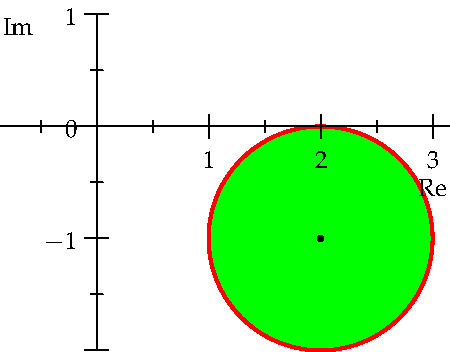
\includegraphics[height=5cm]{6a.pdf}
    \caption{$\abs{z-2+i} \leq 1$ is closed and bounded.}
  \end{figure}

\item
  \begin{figure}
    \centering
    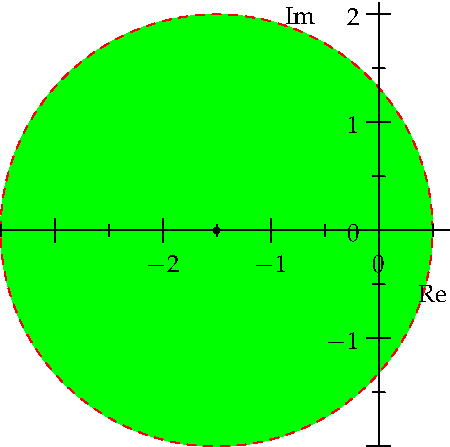
\includegraphics[height=5cm]{6bold.pdf}
    \caption{$\abs{2z+3} < 4$ is bounded, and open and connected so it
      is a domain.}
  \end{figure}

\item
  \begin{figure}
    \centering
    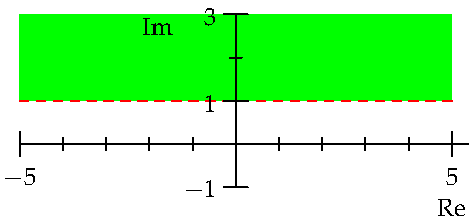
\includegraphics[width=5cm]{6c.pdf}
    \caption{$\Im{z} > 1$ is open and connected, so it is a domain.}
  \end{figure}

\item
  \begin{figure}
    \centering
    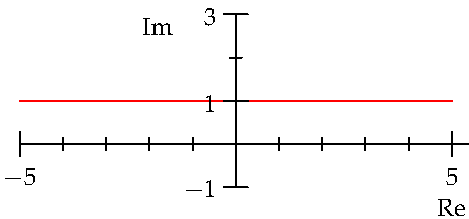
\includegraphics[width=5cm]{6d.pdf}
    \caption{$\Im{z} = 1$ is closed and connected.}
  \end{figure}

\item
  \begin{figure}
    \centering
    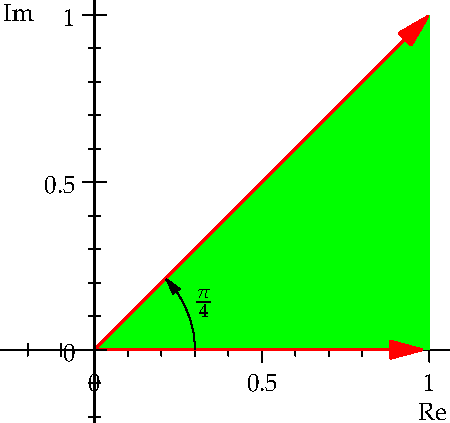
\includegraphics[width=5cm]{6e.pdf}
    \caption{$0 \leq \Arg{z} \leq \frac{\pi}{4}$ with $z \neq 0$ is
      closed and connected}
  \end{figure}
\end{enumerate}


\end{document}

%%% Local Variables:
%%% mode: latex
%%% TeX-master: t
%%% End:
